\documentclass[11pt,a4paper]{report}
\usepackage{marvosym}

\assignment{3}
\group{052}
\students{Bette Jonas}{Huet Anatole}

\begin{document}

\maketitle

\section{Search Algorithms and their relations (3 pts)}
Consider the maze problems given on Figure 1. The goal is to find a path from \Gentsroom ~ to \EURhv ~ moving up, down, left or right. The black cells represent walls. This question must be answered by hand and doesn't require any programming.

\begin{enumerate}
\item Give a consistent heuristic for this problem. Prove that it is consistent. Also prove that it is admissible. \textbf{(1 pt)}
\end{enumerate}

\begin{answers}[4cm]
    % Your answer here
	A consistent heuristic could be to take every legal neighboor (not a wall) of the current cell that we didn't visited yet and calculate the manhattan distance to the goal. We then take the minimum of these distances when we arrive to a cell already visited. 
	
	This heuristic is consistent because the manhattan distance is always positive and the minimum of positive numbers is also positive. Even more, in the best case, the calculated score would be the same as the cost of the shortest path.
	
	It is also admissible because the manhattan distance is the shortest distance between two points in a grid and we are not overestimating the distance to the goal.

    %We take the square that brings us closest to the destination square until we land on it. If there's a wall, we go around it to the right while testing if there's a square that brings us closer to the goal after bypassing the wall. If we come across a square we've already visited, it means we're in a dead end, so we bypass the wall while ignoring the distance to the goal.

    %The character will thus first bypass the wall below them and continue their path until reaching the second wall. They will once again bypass it downwards because they're bypassing to the right and will continue along the wall until reaching where there's a gap. From there, it's a straight line and they reach the destination.
\end{answers}



\begin{enumerate}
\setcounter{enumi}{1}
\item Show on the left maze the states (board positions) that
are visited when performing a uniform-cost graph search, by writing the order numbers in the relevant cells. We assume that when different states in the fringe have the smallest value, the algorithm chooses the state with the smallest coordinate $(i,j)$ ($(0,0)$ being the bottom left position, $i$ being the horizontal index and $j$ the vertical one) using a lexicographical order. \textbf{(1 pt)}
\end{enumerate}

\begin{answers}[5.2cm]
% Your answer here
\begin{center}
	\resizebox{5cm}{!}{
		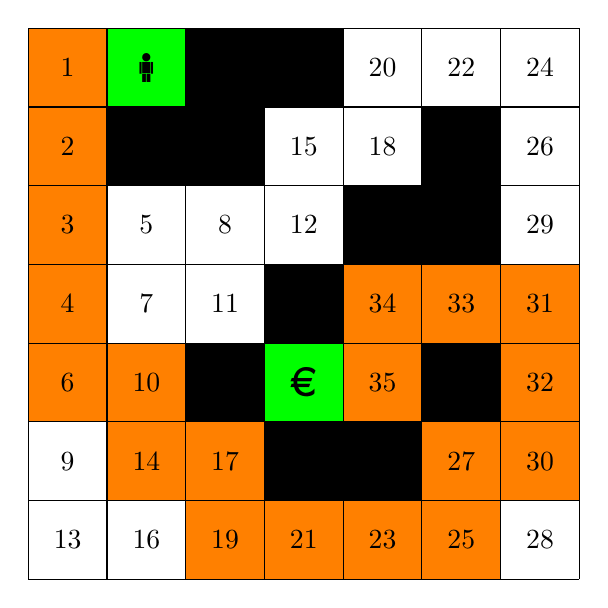
\begin{tikzpicture}
			% Path
			\fill[green] (1, 7) rectangle (2, 6);
			\fill[green] (3, 2) rectangle (4, 3);
			\fill[orange] (0, 7) rectangle (1, 2);
			\fill[orange] (1, 3) rectangle (2, 1);
			\fill[orange] (2, 2) rectangle (3, 0);
			\fill[orange] (3, 1) rectangle (6, 0);
			\fill[orange] (4, 4) rectangle (7, 1);

			\draw (0,0) grid (7, 7);
			
			\fill (2, 7) rectangle (4, 6);
			\fill (1, 6) rectangle (2, 5);
			\fill (2, 7) rectangle (3, 5);
			\fill (4, 5) rectangle (6, 4);
			\fill (5, 6) rectangle (6, 4);
			\fill (3, 4) rectangle (4, 3);
			\fill (2, 3) rectangle (3, 2);
			\fill (3, 2) rectangle (5, 1);
			\fill (5, 2) rectangle (6, 3);
				
			\node at (1.5, 6.5) {\Large \Gentsroom};
			\node at (3.5, 2.5) {\Large \EURhv};
			
			% Numbers
			\node at (0.5, 6.5) {1};
			\node at (0.5, 5.5) {2};
			\node at (0.5, 4.5) {3};
			\node at (0.5, 3.5) {4};
			\node at (1.5, 4.5) {5};
			\node at (0.5, 2.5) {6};
			\node at (1.5, 3.5) {7};
			\node at (2.5, 4.5) {8};
			\node at (0.5, 1.5) {9};
			\node at (1.5, 2.5) {10};
			\node at (2.5, 3.5) {11};
			\node at (3.5, 4.5) {12};
			\node at (0.5, 0.5) {13};
			\node at (1.5, 1.5) {14};
			\node at (3.5, 5.5) {15};
			\node at (1.5, 0.5) {16};
			\node at (2.5, 1.5) {17};
			\node at (4.5, 5.5) {18};
			\node at (2.5, 0.5) {19};
			\node at (4.5, 6.5) {20};
			\node at (3.5, 0.5) {21};
			\node at (5.5, 6.5) {22};
			\node at (4.5, 0.5) {23};
			\node at (6.5, 6.5) {24};
			\node at (5.5, 0.5) {25};
			\node at (6.5, 5.5) {26};
			\node at (5.5, 1.5) {27};
			\node at (6.5, 0.5) {28};
			\node at (6.5, 4.5) {29};
			\node at (6.5, 1.5) {30};
			\node at (6.5, 3.5) {31};
			\node at (6.5, 2.5) {32};
			\node at (5.5, 3.5) {33};
			\node at (4.5, 3.5) {34};
			\node at (4.5, 2.5) {35};
		\end{tikzpicture}
	}
\end{center}
\end{answers}



\begin{enumerate}
\setcounter{enumi}{2}
\item Show on the right maze the board positions visited by $A^{\star}$ graph search with a manhattan distance heuristic (ignoring walls), by writing the order numbers in the relevant cells. A state is visited when it is selected in the fringe and expanded. When several states have the smallest path cost, they are visited in the same lexicographical order as the one used for uniform-cost graph search. \textbf{(1 pt)}
\end{enumerate}

\begin{answers}[5.2cm]
% Your answer here
\begin{center}
	\resizebox{5cm}{!}{
		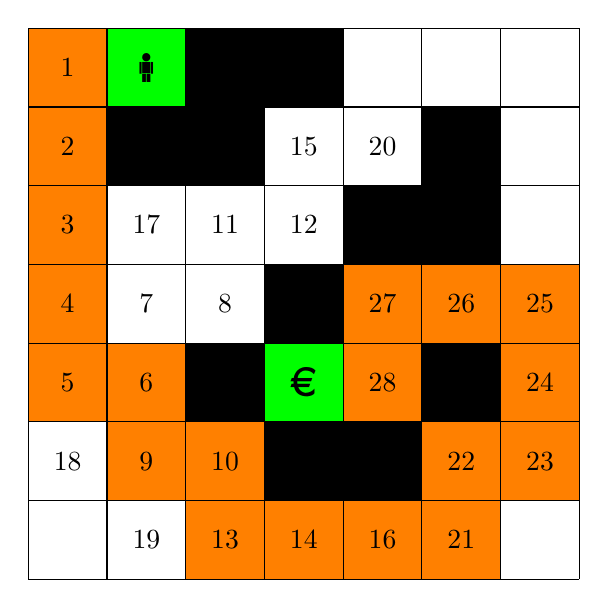
\begin{tikzpicture}
			% Path
			\fill[green] (1, 7) rectangle (2, 6);
			\fill[green] (3, 2) rectangle (4, 3);
			\fill[orange] (0, 7) rectangle (1, 2);
			\fill[orange] (1, 3) rectangle (2, 1);
			\fill[orange] (2, 2) rectangle (3, 0);
			\fill[orange] (3, 1) rectangle (6, 0);
			\fill[orange] (4, 4) rectangle (7, 1);

			\draw (0,0) grid (7, 7);
			
			\fill (2, 7) rectangle (4, 6);
			\fill (1, 6) rectangle (2, 5);
			\fill (2, 7) rectangle (3, 5);
			\fill (4, 5) rectangle (6, 4);
			\fill (5, 6) rectangle (6, 4);
			\fill (3, 4) rectangle (4, 3);
			\fill (2, 3) rectangle (3, 2);
			\fill (3, 2) rectangle (5, 1);
			\fill (5, 2) rectangle (6, 3);
				
			\node at (1.5, 6.5) {\Large \Gentsroom};
			\node at (3.5, 2.5) {\Large \EURhv};

			% Numbers
			\node at (0.5, 6.5) {1};
			\node at (0.5, 5.5) {2};
			\node at (0.5, 4.5) {3};
			\node at (0.5, 3.5) {4};
			\node at (0.5, 2.5) {5};
			\node at (1.5, 2.5) {6};
			\node at (1.5, 3.5) {7};
			\node at (2.5, 3.5) {8};
			\node at (1.5, 1.5) {9};
			\node at (2.5, 1.5) {10};
			\node at (2.5, 4.5) {11};
			\node at (3.5, 4.5) {12};
			\node at (2.5, 0.5) {13};
			\node at (3.5, 0.5) {14};
			\node at (3.5, 5.5) {15};
			\node at (4.5, 0.5) {16};
			\node at (1.5, 4.5) {17};
			\node at (0.5, 1.5) {18};
			\node at (1.5, 0.5) {19};
			\node at (4.5, 5.5) {20};
			\node at (5.5, 0.5) {21};
			\node at (5.5, 1.5) {22};
			\node at (6.5, 1.5) {23};
			\node at (6.5, 2.5) {24};
			\node at (6.5, 3.5) {25};
			\node at (5.5, 3.5) {26};
			\node at (4.5, 3.5) {27};
			\node at (4.5, 2.5) {28};
		\end{tikzpicture}
	}
\end{center}
\end{answers}




\section{N-Amazons problem (8 pts)}

\begin{enumerate}
  \item Model the N problem as a search problem; describe: \textbf{(2 pts)}
		\begin{itemize}
			\item States
			\item Initial state
			\item Actions / Transition model
			\item Goal test
			\item Path cost function
		\end{itemize}
\end{enumerate}

\begin{answers}[8cm]
	% Your answer here
	\underline{States:} A state is represented as an N-element array, where a value of r in the c-th entry means there is an empress at column c, row r, and a value of -1 means that the c-th column has not been filled in yet.
	
	\hspace{0.5cm}
	
	\underline{Initial State:} an  array filled with -1 meaning no pieces has been placed on the board yet.
	
	\hspace{0.5cm}
	
	\underline{Actions:} A piece is being placed on the c-th column of row r.
	
	\hspace{0.5cm}
	
	\underline{Goal test:} Every row has a piece and no pieces can be eaten by another.
	
	\hspace{0.5cm}
	
	\underline{Path Cost Reduction:} The number of conflicts (the bigger it is, the worst it is)
\end{answers}


\newpage
\begin{enumerate}
\setcounter{enumi}{1}
\item Give an upper bound on the number of different states for an N-Amazons problem with N=n. Justify your answer precisely. \textbf{(0.5 pt)}
\end{enumerate}

\begin{answers}[5cm]
	% Your answer here
	The upper bound is N!
	
	\hspace{0.5cm}
	
	For the first queen, there are N choices for its row and N choices for its column. Once the position of the first queen is fixed, the second queen cannot be placed in the same row, column, or diagonal as the first queen. This leaves (N-1) choices for the row and (N-1) choices for the column for the second queen. Similarly, for each subsequent queen, the number of available choices reduces by 1 in each direction (row, column, and diagonals) due to the constraints.
\end{answers}



\begin{enumerate}
\setcounter{enumi}{2}
\item Give an admissible heuristic for a N=n. Prove that it is admissible. What is its complexity ? \textbf{(1 pts)}
\end{enumerate}

\begin{answers}[5cm]
	% Your answer here
	An admissible heuristic is counting the number of pawn that is attacked. The goal is therefore with a heuristic which value is zero.
	\\
	Since each pair of attacking queens represents at least one move that needs to be made to resolve the conflict (either by moving one of the queens or by adding blocking queens), the total number of conflicting pairs serves as a lower bound on the number of moves needed to reach a goal state. Therefore, it is admissible.
	
	\hspace{0.5cm}
	
	This heuristic is efficient to compute and provides a reasonable estimate of the minimum number of moves required to reach a goal state, making it suitable for guiding search algorithms like A* search in the N-Queens problem. It is in O(N*N*N) as for each pieces we need to check if there are any conflicts in the matrix.
\end{answers}



\begin{enumerate}
\setcounter{enumi}{4}
\item \textbf{Implement} your solver. Extend the \emph{Problem} class and implement 
		the necessary methods and other class(es) if necessary.  \textbf{(0.5 pt)}
\item \textbf{Experiment}, compare and analyze informed (\emph{astar\_graph\_search}), uninformed \\
    (\emph{breadth\_first\_graph\_search} and \emph{depth\_first\_graph\_search}) graph search of aima-python3 on N = [10, 11, 12, 13, 20, 25, 30]. \textbf{(3 pts for the whole question)}
		
		Report in a table the time and the number of explored nodes and the number of 
		steps to reach the solution.
		
		Are the number of explored nodes always smaller with 
		\emph{astar\_graph\_search}? 
		What about the computation time? 
		Why? 
		 
		 When no solution can be found by a strategy in a reasonable time (say \textbf{3 
		 min}), indicate the reason (time-out and/or exceeded the memory).
\end{enumerate}

\begin{answers}[8cm]
	% Your answer here
	We decided to run for N on instance 1 With NS = number of paths expanded \& EN = number in frontier.
	
	\hspace{0.5cm}
	
	BFS is really bad for this case as there are a lot of different states to explore. DFS works well for small board size but times out after because it extends its solution based on every action it did. A* is an optimized version of DFS by using an heuristic wich gives a priority of the next state to explore.
\end{answers}

~ 

\begin{answers}[6.5cm]
	\begin{center}
		\begin{tabular}{||l||l|l|l||l|l|l||l|l|l||l|l|l||}
		\hline
		\multirow{3}{*}{N} & \multicolumn{3}{c||}{$A^{\star}$ Graph}& \multicolumn{3}{c||}{BFS Graph} & \multicolumn{3}{c||}{DFS Graph}\\
		& NS & T(s) & EN & NS & T(s) & EN & NS & T(s) & EN\\
		\hline
		10 & 313 & 0.02169 & 14 & 2298 & 0.1533 & 29 & 325 & 0.0075 & 17 \\
		\hline
		11 & 22 & 0.003 & 22 & 7149 & 1.075 & 181 & 24 & 0.00079 & 26\\
		\hline
		12 & 28 & 0.02188 & 88 & 23923 & 21.9423 & 526 & 173 & 0.006 & 26 \\
		\hline
		13 & 502 & 0.06 & 30 & 87922 & 361.88 & 1308 & 107 & 0.0046 & 38 \\
		\hline
		20 & 28 & 0.01889 & 88 & TO & TO & TO & 51861 & 3.9636 & 80\\
		\hline
		25 & 47915 & 20.65 & 125 & TO & TO & TO & 319795 & 37.077 & 147\\
		\hline
		30 & 214187 & 128.36 & 202 & TO & TO & TO & TO & TO & TO\\
		\hline
		\end{tabular}\\
	~\\
	\textbf{NS}: Number of steps — \textbf{T}: Time — \textbf{EN}: Explored nodes — \textbf{TO}: Time-out
	\end{center}
\end{answers}



\begin{enumerate}
\setcounter{enumi}{5}
\item \textbf{Submit} your program on INGInious, using the \textit{A*} algorithm with your best heuristic(s).
		 Your file must be named \emph{namazon.py}. 
      Your program should be able to, given an integer as argument, return the correct output.
		 Your program must print to the standard output a solution to the N's given in argument for the N-Amazons problem, satisfying the described output format. \textbf{(2 pts)}
\end{enumerate}

\begin{answer}
% ANY COMMENTS ABOUT YOUR CODE
\end{answer}

\section{Local Search: Sudoku Problem (8 pts)}

\begin{enumerate}
    \item Formulate the Sudoku problem as a Local Search problem (problem, cost function, feasible solutions, optimal solutions). \textbf{(2 pts)}
\end{enumerate}

\begin{answer}
	% Your answer here
	\underline{Problem:} Find a solution to a Sudoku puzzle.
	\\
	\underline{Cost Function:} The cost function is the number of conflicts in the board.
	\\
	\underline{Feasible Solutions:} A feasible solution is a board where no conflicts are present.
	\\
	\underline{Optimal Solutions:} An optimal solution is a board where no conflicts are present and all the numbers are placed correctly.
\end{answer}

\begin{enumerate}
    \item You are given a template on Moodle: \url{sudoku.py}. Implement your own simulated annealing algorithm and your own \url{objective\_score} function. Your program will be evaluated in on 15 instances (during 3 minutes each) of which 5 are hidden. We expect you to solve (get the optimal solution) at least 12 out of the 15. \textbf{(6 pt)}
\end{enumerate}

\begin{answer}
 % ANY COMMENTS ABOUT YOUR CODE
\end{answer}

\end{document}